\documentclass[12pt]{article}

%VARIABLES
\def \geometryDefault {
	a4paper,
	left=35mm,
	right=20mm,
	top=25mm,
	bottom=25mm
}
\def \geometryTitlePage {
	left=25mm,
	right=25mm,
	top=25mm,
	bottom=25mm
}
\def \geometryGraduationCard {
	left=25mm,
	right=10mm,
	top=25mm,
	bottom=25mm
}
\def \geometryStatement {
	left=25mm,
	right=10mm,
	top=25mm,
	bottom=25mm
}

%page settings
\usepackage[\geometryDefault]{geometry}% margins
\usepackage{times} % Times New Roman
\setlength{\parindent}{1cm} % tab indentation
\linespread{1.5} % interline
\usepackage{indentfirst} % tab the first line in a section

%language settings
\usepackage[utf8]{inputenc}
\usepackage[T1]{fontenc}
\usepackage[polish]{babel}
\usepackage{csquotes}
\DeclareQuoteAlias{croatian}{polish} % croatian has the same properties as polish

%code options
\usepackage{listings}
\usepackage{xcolor}

\colorlet{punct}{red!60!black}
\definecolor{delim}{RGB}{20,105,176}
\colorlet{numb}{magenta!60!black}

\lstdefinelanguage{json}{
    basicstyle=\normalfont\ttfamily,
    %numbers=left,
    numberstyle=\scriptsize,
    stepnumber=1,
    frame=single,
    %showstringspaces=false,
    breaklines=true,
    captionpos=b,
    escapeinside={\%*}{*)},
    literate={ą}{{\k{a}}}1
             {Ą}{{\k{A}}}1
             {ę}{{\k{e}}}1
             {Ę}{{\k{E}}}1
             {ó}{{\'o}}1
             {Ó}{{\'O}}1
             {ś}{{\'s}}1
             {Ś}{{\'S}}1
             {ł}{{\l{}}}1
             {Ł}{{\L{}}}1
             {ż}{{\.z}}1
             {Ż}{{\.Z}}1
             {ź}{{\'z}}1
             {Ź}{{\'Z}}1
             {ć}{{\'c}}1
             {Ć}{{\'C}}1
             {ń}{{\'n}}1
             {Ń}{{\'N}}1
}

\renewcommand\lstlistingname{Kod źródłowy}
\renewcommand{\lstlistlistingname}{Kody źródłowe}

%Here I change numeric pattern to include chapter number
\usepackage{chngcntr}
\AtBeginDocument{\counterwithin{lstlisting}{section}} %listings
\AtBeginDocument{\counterwithin{figure}{section}} %images

%Make images captions to be on the bottom
%\usepackage{floatrow}

%Define new block, so that if a code is split between 2 pages, then it moves it to the second one.
\lstnewenvironment{code}[1][]%
{
   \noindent\newline
   \minipage{\linewidth} 
   \vspace{0.5\baselineskip}
   \lstset{frame=single,#1}}
{\endminipage}

%images settings
\usepackage{graphicx}

%lorem ipsum
\usepackage{lipsum}

%nomenclature
\usepackage{nomencl}
\makenomenclature

%turn off the warnings
\hfuzz=20pt
\vfuzz=20pt
\hbadness=20000
\vbadness=\maxdimen

%allows referencing sections  to return names, not numbers
\usepackage[hidelinks]{hyperref}


%START
\begin{document}

%TITLE PAGE
\begin{titlepage}
	%\expandafter\newgeometry\expandafter{\geometryTitlepage} % set margins to equal
	
	\begin{center}
		{\scshape 
			{\large Politechnika Białostocka}\par
			\vspace{0.5cm}
			{\large Wydział Informatyki}\par
			\vfill
			{\large <YOUR NAME>}\par
			\vspace{0.4cm}
			.......................................\\
			\begin{small}
				\vspace{-0.2cm}
				(Podpis)  
			\end{small}\par	
			\vspace{2cm}
			{\LARGE
				My fabulous Master Thesis title\par
			}
			\vspace{4cm}
		}
		\begin{flushright}
			{\large
				Praca magisterska\par
				napisana pod kierunkiem\par
				dr <YOUR PROMOTOR'S NAME :)>\par
				\vspace{0.4cm}
				.......................................\\
				\begin{small}
					\vspace{-0.2cm}
					(Podpis)\hspace{1.63cm}    
				\end{small}				   
			}
		\end{flushright}
		\vfill
		{\scshape\large\ Białystok 2018}
	\end{center}
	
	%\restoregeometry % restore margins to default
	
\end{titlepage}


\setcounter{page}{2}

%GRADUATION PAGE (karta dyplomowa)
\expandafter\newgeometry\expandafter{\geometryGraduationCard}
\begin{center}
	{\textbf{Karta dyplomowa}}
	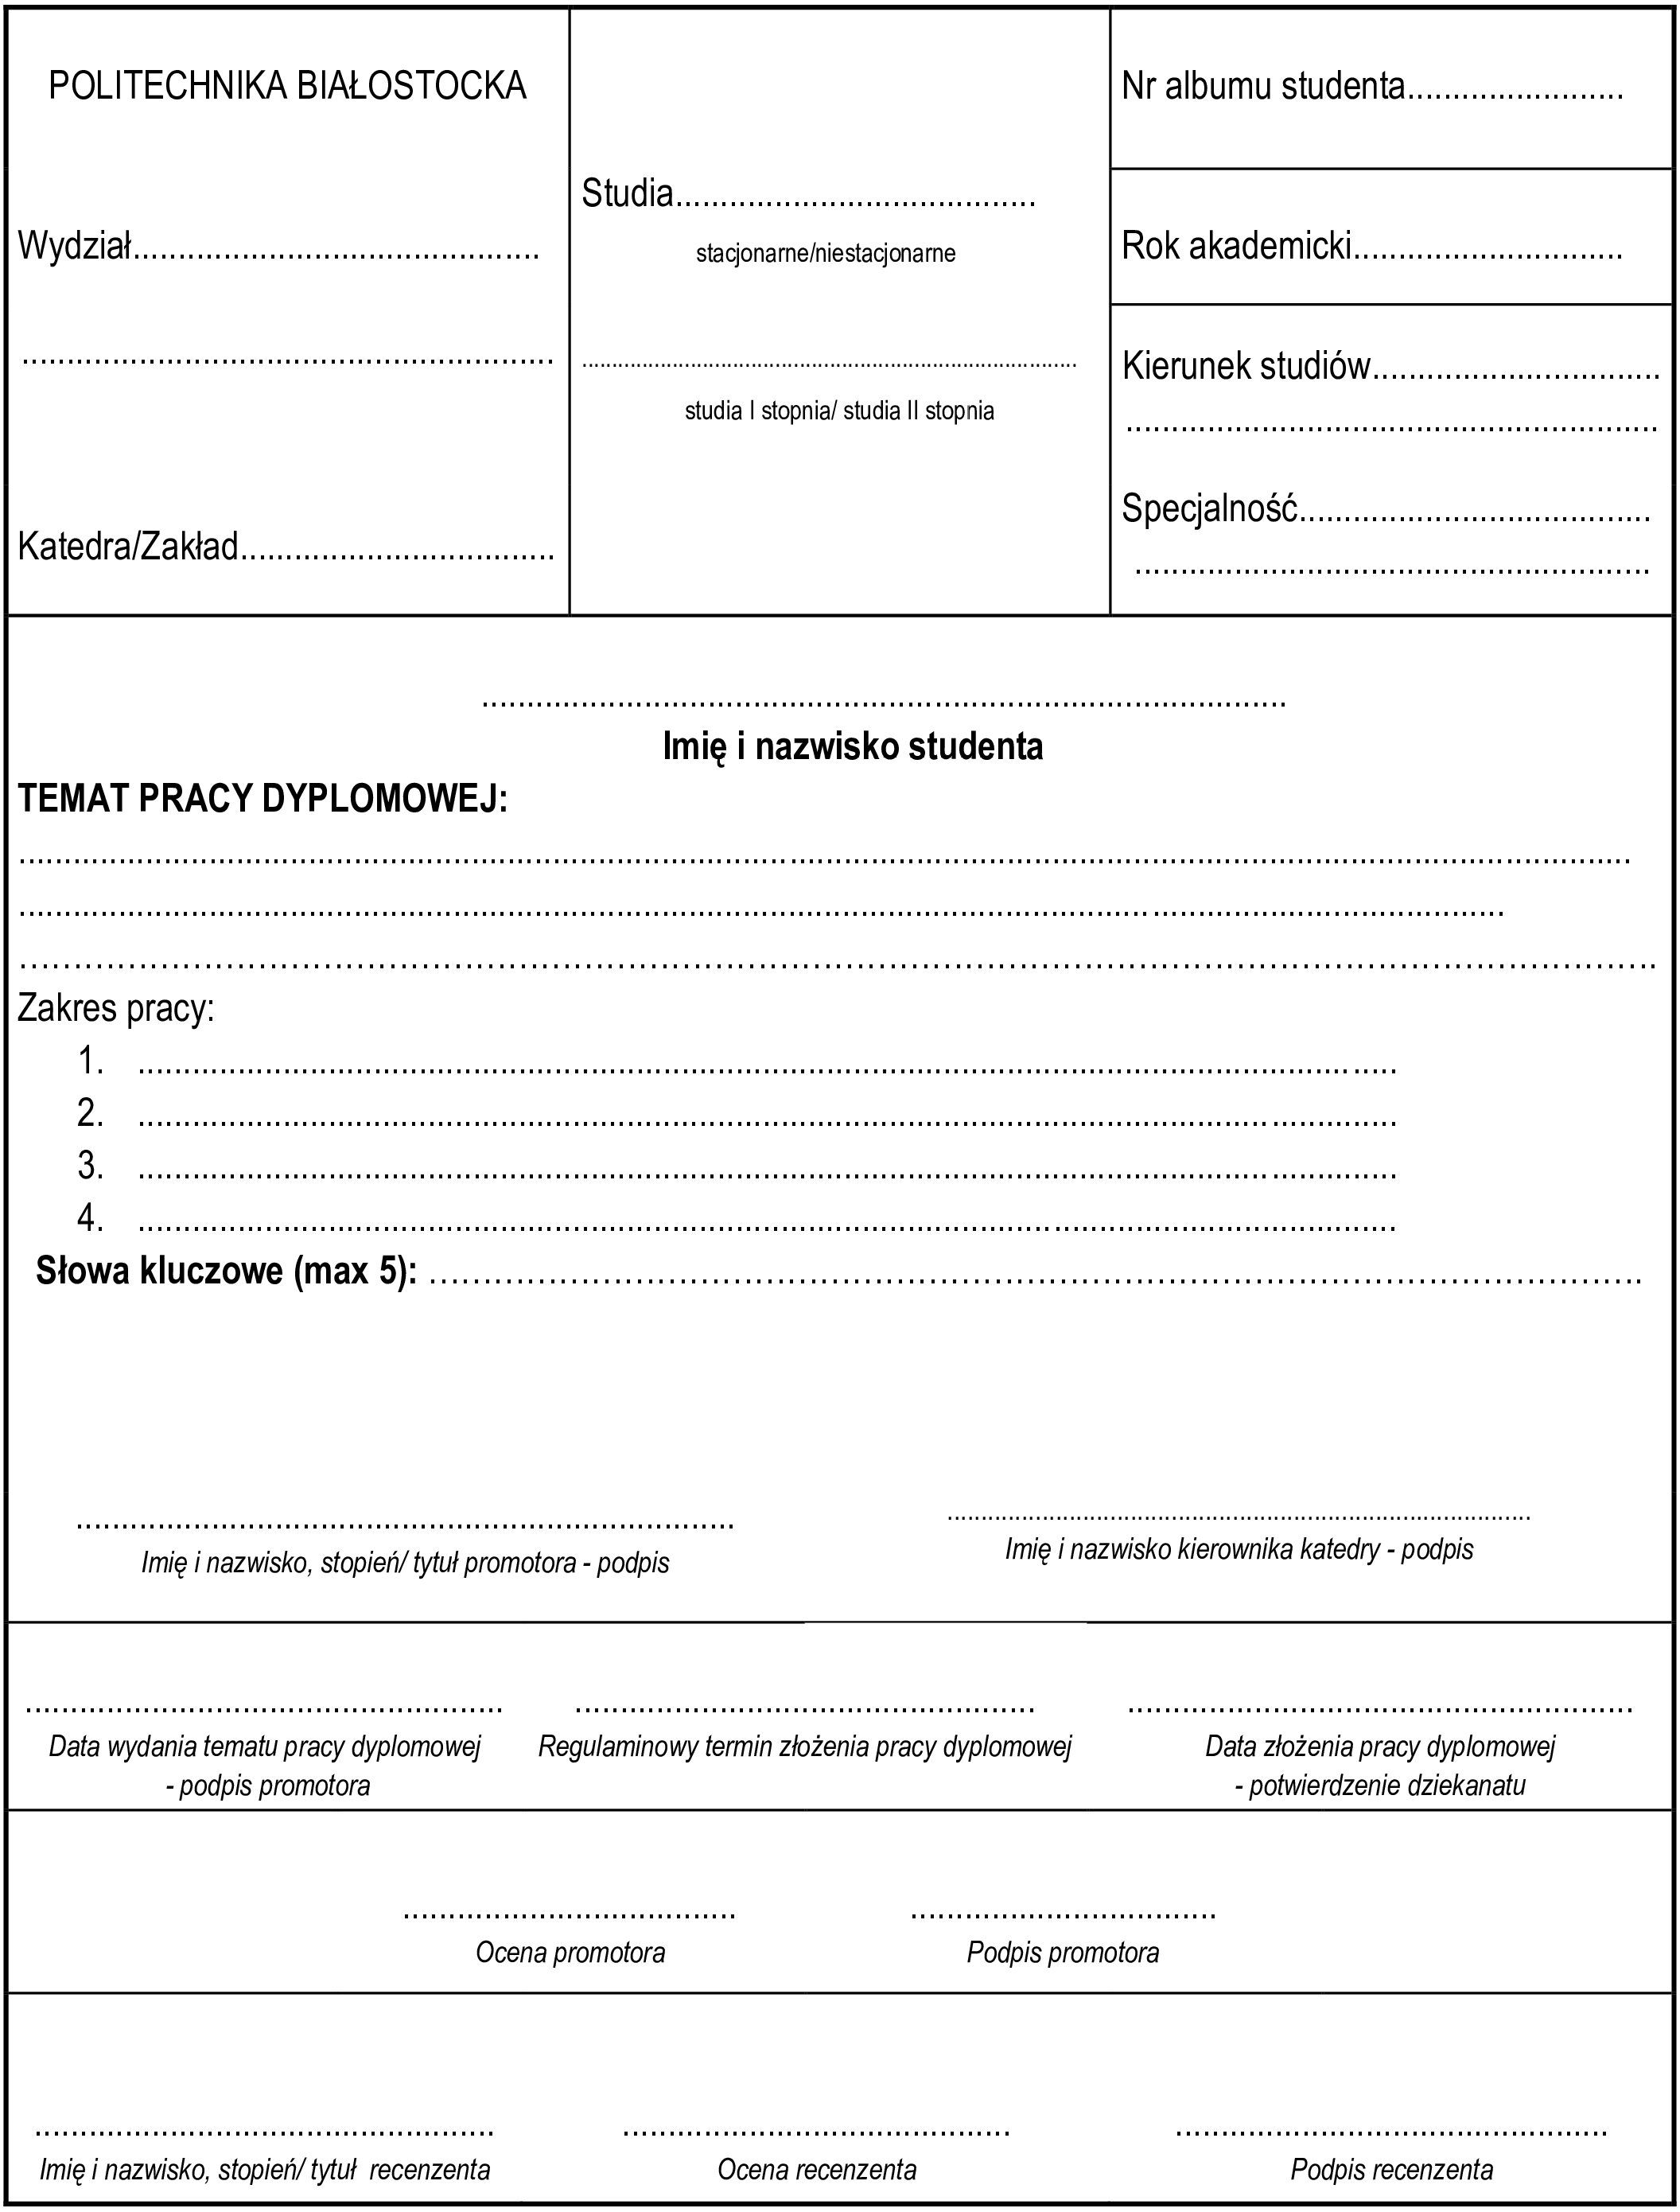
\includegraphics[width=\linewidth]{img/kartaDyplomowa.png}
\end{center}
\restoregeometry

%THESIS SUMMARY
\textbf{Thesis topic}: \textbf{------YOUR NICE THESIS SUMMARY------}  A website to register personal achievements in e-sport games.\par
\textbf{SUMMARY}: The website enables user to create and custimize various tasks to accomplish in one of the supported games (League of Legends, Dota 2). In order to do so a user is required to connect his game account with the account he created on the website using secure authenticating methods. To complete the tasks user must play a match in a selected game and fullfill the required goals. A positive outcome will result in receiving a reward. The application is open to support another games, which must provide a proper Web API.

%STATEMENT
\expandafter\newgeometry\expandafter{\geometryStatement}
\begin{center}
	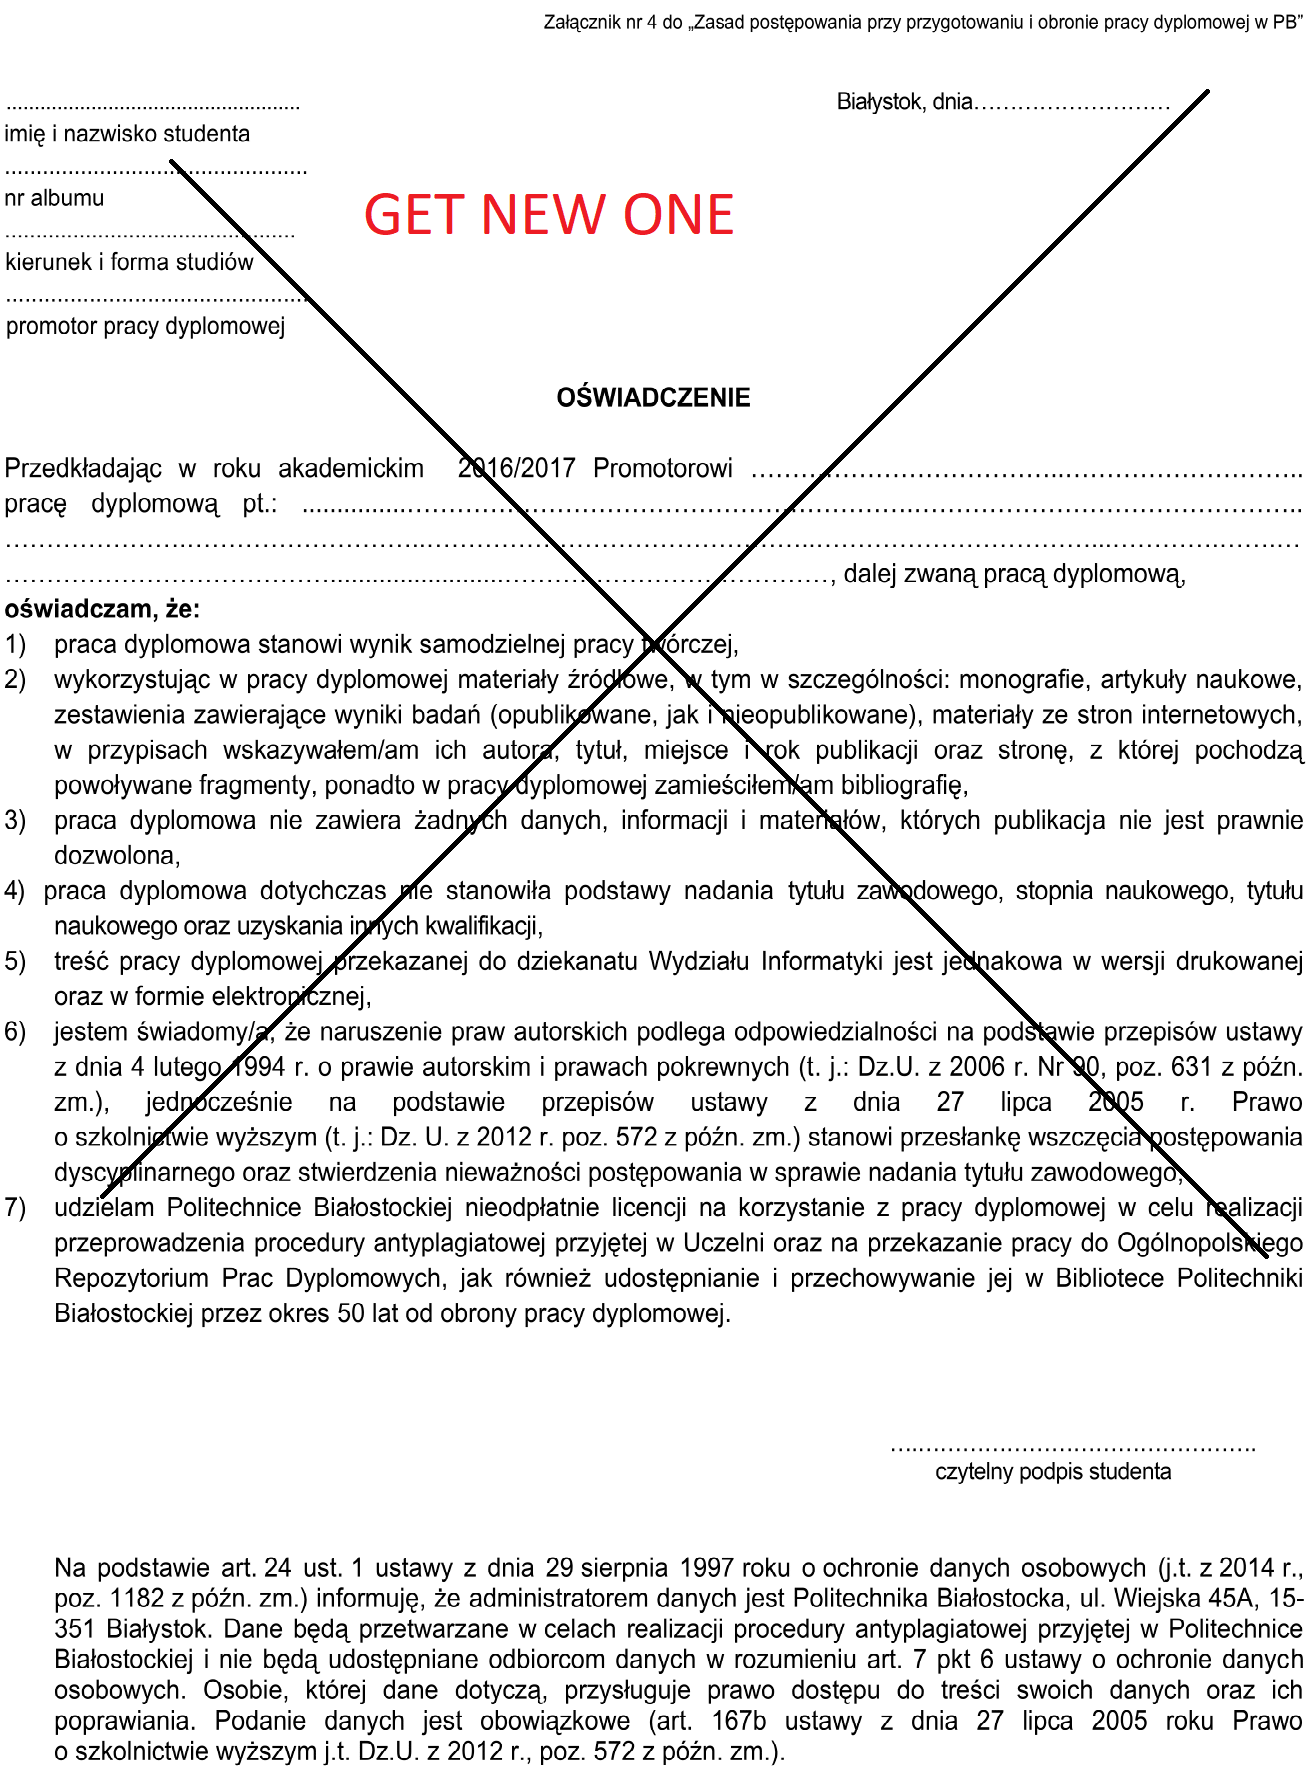
\includegraphics[width=\linewidth]{img/oswiadczenie.png}
\end{center}
\restoregeometry

%TABLE OF CONTENTS (spis treści)
\tableofcontents

%-----------------YOUR CONTENT STARTS HERE-------------------
\section{Wstęp}
	W latach 90 dwudziestego wieku gry komputerowe zaczęły budzić zainteresowanie coraz większej ilości osób między innymi z powodu wprowadzania tytułów posiadających grafikę w trójwymiarze (3D). Był to kamień milowy, który udowodnił, że istnieje możliwość odtworzenia rzeczywistości w świecie wirtualnym. Niestety, ograniczeniem była wtedy wydajność sprzętowa.\par
	Dziś, dwie dekady później, technologia jest na bardzo wysokim poziomie. Powstały gry takie jak \textit{Grand Theft Auto V}, czy \textit{Wiedźmin 3: Dziki Gon}, które zachwycają oprawą graficzną, rozgrywką, muzyką oraz pozwalają graczowi poczuć, że niekiedy tamta, wirtualna rzeczywistość, bywa bardziej realistyczna od tej prawdziwej.\par
	Przeskok technologiczny i rozwój Internetu pozwoliły nie tylko na granie w pojedynkę (singleplayer), ale również na rozgrywkę z innymi (multiplayer). To, w połączeniu z ludzką naturą, chęcią rywalizacji, utworzyło nową kategorię sportu o nazwie \blockquote{e-sport}.\par
	E-sport jest formą rywalizacji, która odbywa się za pośrednictwem gier komputerowych. Jej głównym celem jest wygrana którą można osiągnąć tylko dzięki taktyce i koordynacji drużyny. Aby uzyskać odpowiedź dlaczego e-sport jest tak popularny należy zadać pytanie: Dlaczego piłka nożna jest najpopularniejszą dyscypliną sportu na świecie? \cite{footballPopularity} W odróżnieniu, np. od hokeja, który wymaga lodu, łyżew, krążka, kija i ochraniaczy, aby zagrać w piłkę nożną wystarczy bardzo niewiele: piłka i dwa słupki. Istnieje teoria zwana \textit{Prawem Bushnell-a}, która brzmi następująco:
	\begin{center}
		\blockquote{All the best games are easy to learn and difficult to master.} \cite{burshnellsLaw}
	\end{center}
Co w wolnym tłumaczeniu znaczy, że najlepsze gry to takie, które są proste w nauce, jednak trudne w opanowaniu. Taka właśnie jest piłka nożna i taki jest e-sport, gdzie aby naśladować profesjonalistę wystarczą jedynie chęci.\par
	Profesjonalni sportowcy muszą liczyć się z naturalnym zmęczeniem organizmu, dlatego trenują tylko kilka godzin dziennie. Natomiast profesjonalni \blockquote{e-sportowcy}, aby być w światowej czołówce trenują często po 12 godzin dziennie lub więcej. \cite{proPlayerPlayTime} Czas ten nieznacznie różni się w przypadku zwykłych graczy komputerowych. Oczywiście, część gra 2 godziny, a część spędza cały dzień. Nie zmienia to jednak faktu, że w obu tych przypadkach po pewnym czasie zaczyna się odczuwać monotonię. Sama wygrana przestaje być celem nadrzędnym. Przez to cierpi nie tylko sam gracz, ale i jego zespół, który nie będąc w pełni zgranym staje się bardziej podatny na porażkę.\par
	\subsection*{Cel pracy}
		Aby rozwiązać problem znudzenia i braku efektywności w rozgrywce celem pracy jest zmotywowanie gracza do wygranej oraz polepszenie jego umiejętności poprzez wykonywanie zadań. Zadania nie zagwarantują wygranej, lecz w mniejszym lub większym stopniu do niej przybliżą. Użytkownik będzie miał możliwość tworzenia i personalizowania zadań do wykonania w wybranych grach. Określić będzie mógł ile razy ma je wykonać oraz do kiedy. Aby móc sprawdzić czy zadanie zostało wykonane w pierwszej kolejności musi rozegrać prawdziwy mecz w wybranej grze.\par
	
	
	

%IMPLEMENTATION PROCESS
\section{Proces implementacji}

\subsection{Połączenie z kontem gry}
		Załóżmy, że użytkownik tej aplikacji będzie chciał wykonać kilka zadań w nadchodzących meczach. W tym celu musi podać nazwę swojego konta po to, aby serwer mógł pobierać odpowiednią historię meczów. Jednak w tym miejscu pojawia się problem. Co, jeśli ktoś poda nazwę nieswojego konta? Będzie wtedy czerpał korzyści z cudzych osiągnięć, a prawowity właściciel nie będzie nic z tego miał. Rozwiązaniem musi być więc potwierdzenie posiadania konta.\par
	\subsubsection{League of Legends}
			Niestety, League of Legends nie posiada takiego mechanizmu. Kuszącą propozycją byłoby pobranie od użytkownika loginu i hasła i zdalne zalogowanie się na jego konto w celu sprawdzenia wiarygodności. Ten pomysł jednak naruszałby zasady bezpieczeństwa. W razie wykrycia, aplikacja zostałaby dożywotnio zablokowana. Innym aspektem jest to, że jeśli jakaś aplikacja prosi o dane logowania na inną domenę, to można z wysokim prawdopodobieństwem założyć, że w ten sposób spróbuje włamać się na te konto.\par
			Innym podejściem byłoby wykonanie określonej czynności, do której tylko właściciel miałby dostęp. Każde konto w League of Legends posiada zbiór stron zwanych \blockquote{Mastery Pages}. Jest to lista maksymalnie 20 stron z ustawieniami gracza, z której każda może zostać nazwana indywidualnie. To, plus fakt, że API udostępnia URI, które zwraca ich całą listę powoduje, że sposób ten stał się rozwiązaniem jak połączyć konto aplikacji z kontem League of Legends.\par
			Po wypełnieniu i wysłaniu formularza (rysunek \ref{img:exampleImage}) serwer sprawdza, czy takie konto istnieje w podanym regionie oraz czy inny użytkownik nie ma przypisanego konta o tej nazwie. W przypadku, gdy obie wersje się potwierdzą, użytkownik zostanie przekierowany na stronę z obecnym statusem (rysunek \ref{img:exampleImage}). Na niej zostanie poinformowany jak musi nazwać jedną ze swoich Mastery Page. Po nazwaniu strony i wciśnięciu przycisku do weryfikacji status konta zostanie zaktualizowany (rysunek \ref{img:exampleImage}).\\
\begin{figure}[!ht]
	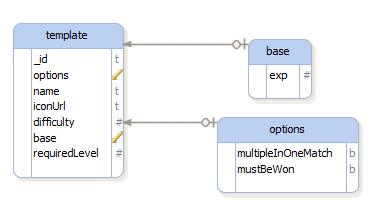
\includegraphics[width=\linewidth]{img/exampleImage}
	\caption{Example caption}
	\label{img:exampleImage}
\end{figure}	

\subsection{Wielojęzyczność}
	Gry e-sportowe nie ograniczają się do wąskiej grupy ludzi z jednego kraju. Zrzeszają graczy z całego świata, którzy często znają tylko jeden język. Dlatego gry te posiadają wsparcie dla wielu języków, ponieważ użytkownik nie będzie szukał gry, do której będzie się musiał dostosować, a raczej takiej, która się dostosuje do niego. W tej aplikacji również nie ograniczono się do jednego języka, a rozszerzalność na kolejne odbywa się na zasadzie przetłumaczenia pliku z tłumaczeniami i dodanie w opcjach nowego języka.

	\subsubsection*{Biblioteka \blockquote{angular-translate}}
		Do wprowadzenia wielojęzyczności użyta została biblioteka \blockquote{angular-translate} \cite{ref:angularTranslateDoc}. Jest to moduł do frameworka AngularJS, który ma przydatne w użyciu dyrektywy, filtry i serwisy, oraz posiada fazę konfiguracji, w której można spersonalizować działanie za pomocą dostępnych opcji.\par
		 Podczas startu aplikacji, aby wybrać język, w pierwszej kolejności sprawdzany jest Local Storage. Następnie sprawdzany jest obecny język przeglądarki. Jeśli obie te metody zawiodą, to wybrany zostaje język domyślny (angielski). Nowo wybrany język jest automatycznie zapisywany do Local Storage.\par
		 Każdy język posiada tłumaczenie w oddzielnym pliku w formacie JSON. Rozdziela to funkcjonalność od reszty kodu w aplikacji. Inną zaletą jest ułatwienie zarządzania treścią, ponieważ łatwiej jest manipulować sformułowaniami w jednym pliku, niż w bardzo wielu nieczytelnych widokach HTML. Przykład takiego tłumaczenia można zobaczyć w kodzie źródłowym \ref{lis:translation}. W przypadku braku konkretnego klucza w tłumaczeniu wyświetlany jest komunikat w  docelowym miejscu na stronie oraz w konsoli (kod źródłowy \ref{lis:missingTranslation}). Informuje on o tym, który klucz należy uzupełnić i w jakim języku. Informacja ta jest lokalna, ale w razie rozwoju aplikacji można by w takim wypadku wysyłać ją do serwera, który poinformuje dewelopera o błędach.
		 
\begin{code}[
		language=javascript,
		caption={Problem synchronizacji stanu aplikacji w jQuery (źródło: opracowanie własne)},
		label={lis:jquery-state-sync-problem},
		escapechar=|
	]
var user = { |\label{line:jquery-user}|
  name: "John",
  age: 25
}

function updateDOMUser() { |\label{line:jquery-update-dom}|
  \$("#userName").text(user.name)
  \$("#userAge").text(user.age)
}

user = getNewUser() |\label{line:jquery-user-get}|
updateDOMUser()

	\end{code}\\
	
	W kodzie źródłowym \ref{lis:jquery-state-sync-problem} przedstawiony został ... W linijce \ref{line:jquery-user} widać obiekt usera.
	
\clearpage

\begin{table} % you can add [!ht] here to make this table always float to the top
		\centering
		\caption{Parametry sprzętu, na którym przeprowadzone zostały testy aplikacji webowych (źródło: opracowanie własne)}
		\label{tab:comp-spec}
    	\begin{tabular}{ | l | l |}
    \hline
    Nazwa & Wersja \\ \hline
    Procesor & Intel Core i7-8700k 3,7GHz \\ \hline
    Pamięć RAM & Corsair Venegeance LPX DDR4 3200MHz 32GB \\ \hline
    Dysk twardy & Crucial 250 GB 2,5'' SATA SSD \\ \hline
    System Operacyjny & Windows 10 Educational 64 bit, wersja 1803 \\ \hline
    Przeglądarka & Google Chrome 64 bit, wersja 66.0.3359.181 \\ \hline
    \end{tabular}
\end{table}

	W tabelce \ref{tab:comp-spec} pokazane zostały parametry sprzętu.


%----------------YOUR CONTENT ENDS HERE---------------------

\clearpage
%BIBLIOGRAPHY
\addcontentsline{toc}{section}{Literatura}
\bibliographystyle{IEEEtran}
\bibliography{bib/bibliography}

%NOMENCLATURE
\printnomenclature

%LISTINGS
\clearpage
\pagenumbering{gobble}
\addcontentsline{toc}{section}{Kody źródłowe}
\lstlistoflistings

%DRAWINGS
\clearpage
\addcontentsline{toc}{section}{Spis rysunków}
\listoffigures

\end{document}
